% arara: pdflatex
% arara: pdflatex

\documentclass[xcolor=dvipsnames]{beamer}
\usetheme[
  numbering=fraction,
  % numbering=none,
  sectionpage=progressbar,
  subsectionpage=none,
  % block=fill,
  progressbar=foot,
]{metropolis}
\definecolor{DartGreen}{cmyk}{0.95,0,1,0.50}
\setbeamercolor{progress bar}{fg=DartGreen}
\makeatletter
  \setlength{\metropolis@titleseparator@linewidth}{5pt}
  \setlength{\metropolis@progressonsectionpage@linewidth}{5pt}
  \setlength{\metropolis@progressinheadfoot@linewidth}{5pt}
\makeatother

\usepackage{appendixnumberbeamer}

\usepackage{stmaryrd}
\usepackage{soul}
\usepackage{amssymb,amsthm,amsmath,amsxtra,mathrsfs}
% \usepackage[all]{xy}
% \usepackage{xfrac}
% \usepackage{calc}
\usepackage{tikz}
\usetikzlibrary{arrows,calc,automata,shadows,backgrounds,positioning,intersections,fadings,decorations.pathreplacing,shapes,snakes, matrix}
\usepackage{tikz-cd}
\tikzset{commutative diagrams/.cd, arrow style = tikz, diagrams = {>=latex}}
\tikzset{>=latex}

\usepackage{filecontents}
\usepackage{pgfplots, pgfplotstable}
\usepgfplotslibrary{statistics}

\usepackage{marvosym}
\usepackage[marvosym]{tikzsymbols}
\usepackage{colonequals}

\theoremstyle{plain}
\newtheorem*{thm}{Theorem}
\newtheorem*{lem}{Lemma}
\newtheorem*{prop}{Proposition}
\newtheorem*{ques}{Question}
\newtheorem*{conj}{Conjecture}
\newtheorem*{cor}{Corollary}

% \usecolortheme{owl}
\usecolortheme[snowy]{owl}

\newcommand{\OO}{\mathcal O}
\newcommand{\PP}{\mathbb P}
\newcommand{\CC}{\mathbb C}
\newcommand{\RR}{\mathbb R}
\newcommand{\QQ}{\mathbb Q}
\newcommand{\ZZ}{\mathbb Z}
\renewcommand{\AA}{\mathbb A}
\newcommand{\defi}[1]{\textsf{#1}}
\newcommand{\jv}[1]{{\color{red} \sf JV: [#1]}}
\newcommand{\mm}[1]{{\color{blue} \sf MM: [#1]}}
\newcommand{\wt}[1]{\widetilde{#1}}
\newcommand{\QQal}{{\mathbb Q}^{\textup{al}}}
\newcommand{\FFqal}{{\mathbb F}_q^{\textup{al}}}
\newcommand{\QQab}{{\mathbb Q}^{\textup{ab}}}
\newcommand{\QQbar}{{\mathbb Q}^{\textup{al}}}
\newcommand{\Kal}{{{K}^{\textup{al}}}}
\newcommand{\Kab}{{K}^{\textup{ab}}}
\newcommand{\kbar}{\overline{k}}
\newcommand{\Kbar}{\overline{K}}
\newcommand{\LL}{\mathscr L}
\newcommand{\sm}{\setminus}
\newcommand{\FF}{\mathbb{F}}
\renewcommand{\ker}{\operatorname{ker}}

\DeclareMathOperator{\con}{con}
\DeclareMathOperator{\Div}{Div}
\DeclareMathOperator{\Princ}{Princ}
\DeclareMathOperator{\Pic}{Pic}
\DeclareMathOperator{\ddiv}{div}
\DeclareMathOperator{\sat}{sat}
\DeclareMathOperator{\ddeg}{deg}
\DeclareMathOperator{\ddim}{dim}
\DeclareMathOperator{\rred}{red}
% \renewcommand{\rred}{\operatorname{red}}
\DeclareMathOperator{\Lifts}{Lifts}
\DeclareMathOperator{\order}{order}
\DeclareMathOperator{\Aut}{Aut}
\DeclareMathOperator{\PGL}{PGL}
\DeclareMathOperator{\Mon}{Mon}
\DeclareMathOperator{\Gal}{Gal}
\DeclareMathOperator{\supp}{supp}
\DeclareMathOperator{\ord}{ord}
\DeclareMathOperator{\mult}{mult}
\DeclareMathOperator{\stab}{stab}
\DeclareMathOperator{\orb}{orb}
\DeclareMathOperator{\id}{id}
% \DeclareMathOperator{\ker}{ker}
\DeclareMathOperator{\GL}{GL}
\DeclareMathOperator{\charpoly}{charpoly}
% \DeclareMathOperator{\det}{det}
\DeclareMathOperator{\Tr}{tr}
\DeclareMathOperator{\Pl}{Pl}
\DeclareMathOperator{\Cl}{Cl}
\DeclareMathOperator{\Jac}{Jac}
\DeclareMathOperator{\minpoly}{minpoly}


\title{$2$-group Belyi maps}
\author{Michael Musty}
\date{July 9, 2019}
\institute{Dartmouth College}
\begin{document}
  \maketitle
  \begin{frame}{Outline}
    \tableofcontents
  \end{frame}
  \section{Motivation}{
    \begin{frame}[fragile]{Factoring in number fields}
      Let $F$ be a number field with ring
      of integers $\ZZ_F$.
      \begin{align*}
        \begin{tikzcd}[ampersand replacement=\&]
          \&F\arrow[dash]{dl}\\
          \ZZ_F\arrow[dash]{d}\&\QQ\arrow[dash]{u}\\
          \ZZ\arrow[dash]{ur}
        \end{tikzcd}
        % \quad
        % \quad\quad\quad\quad
        % \begin{tikzcd}[ampersand replacement=\&]
        %   \&\left\{x+y\sqrt{7}:x,y\in\QQ\right\}\arrow[dash]{dl}\\
        %   \left\{a+b\sqrt{7}:a,b\in\ZZ\right\}\arrow[dash]{d}\&\QQ\arrow[dash]{u}\\
        %   \ZZ\arrow[dash]{ur}
        % \end{tikzcd}
      \end{align*}
      \pause
      \[
        p\ZZ_F = \mathfrak{p}_1^{e_1}\cdots\mathfrak{p}_g^{e_g}
      \]
      \pause
      A prime $p\in\ZZ$ is \textbf{ramified} in $F$ if
      $e_i\geq 2$ for some $i$.
      \pause\par
      Does there exist a number field
      where $2$ is the \emph{only} ramified prime?
      \pause
      Nonsolvable?
    \end{frame}
    \begin{frame}[fragile]{Why $2$-group Belyi maps?}
      \begin{center}
        \begin{tikzpicture}[scale=1]
          \node at (4,0) (fieldramifiedonlyattwo)
          {
            $
              % \left\{
                \begin{minipage}{13ex}
                  number fields
                  ramified at $2$
                \end{minipage}
              % \right\}
            $
          };
          \node at (-4,0) (twogroupbelyis)
          {
            $
              % \left\{
                \begin{minipage}{18ex}
                  $2$-group Belyi maps
                \end{minipage}
              % \right\}
            $
          };
          \node at (0,-6) (curveswithgoodreduction)
          {
            $
              % \left\{
                \begin{minipage}{25ex}
                  curves with good reduction
                  away from $p=2$
                \end{minipage}
              % \right\}
            $
          };
          % \draw[->] (twogroupbelyis) to node [above,rotate=35] {Beckmann's theorem} node {} (curveswithgoodreduction);
          \draw[->] (twogroupbelyis) to node [above,rotate=-55.5,blue] {Beckmann's theorem} node {} (curveswithgoodreduction);
          \draw[->] (curveswithgoodreduction) to node [above,rotate=55.5,blue] {N\'{e}ron-Ogg-Shafaravich} node {} (fieldramifiedonlyattwo);
          \draw[dashed,->] (twogroupbelyis) to node [above] {} node {} (fieldramifiedonlyattwo);
        \end{tikzpicture}
      \end{center}
    \end{frame}
    \begin{frame}{Why $p=2$?}
      \begin{conj}[Gross 1998]
        \vspace{1pt}
        For every prime $p$,
        there exists a nonsolvable Galois number field
        ramified only at $p$.
      \end{conj}
      \pause
      $p\geq 11$ : existence (Serre), explicit (Edixhoven, Mascot)
      \par
      $p=7$ : existence (Dieulefait, Roberts)
      \par
      $p=5$ : existence (Demb\'{e}l\'{e}, Greenberg, Voight), explicit (Roberts)
      \par
      $p=3$ : existence (Demb\'{e}l\'{e}, Greenberg, Voight)
      \par
      $p=2$ : existence (Demb\'{e}l\'{e})
      \pause
      \par
      The hope is that an explicit nonsolvable field ramified only at $2$
      can be obtained as $K(\Jac(X)[2])$ where
      $X$ is the domain of a
      \textbf{$2$-group Belyi map}
      (which we will define shortly).
    \end{frame}
    \begin{frame}{Main results}
      Motivated by the applications of
      $2$-group Belyi maps to arithmetic geometry,
      we now state the main results.
      \pause
      \begin{itemize}
        \item
          implementation of an algorithm to
          enumerate isomorphism classes
          of $2$-group Belyi maps
          \pause
        \item
          implementation of an algorithm to
          compute equations for
          $2$-group Belyi maps
          over finite fields
          \pause
        \item
          implementation of a \emph{method}
          to compute equations for
          $2$-group Belyi maps
          over number fields
          \pause
        \item
          computational and theoretical evidence
          supporting a conjecture that
          every $2$-group Belyi map
          is defined over an
          abelian extension of the rationals
      \end{itemize}
    \end{frame}
  }
  \section{Background}{
    \begin{frame}{Belyi's theorem}
      A \textbf{Belyi map}
      is a morphism
      $\phi\colon X\to\PP^1$
      of smooth projective algebraic curves
      over $\CC$
      that is unramified outside of
      $\{0,1,\infty\}$.
      \pause
      \begin{thm}[Belyi 1979]
        \vspace{1pt}
        An algebraic curve (smooth projective)
        $X$ over $\CC$ can be defined over a number
        field if and only if $X$ admits a
        Belyi map.
      \end{thm}
    \end{frame}
    \begin{frame}{$2$-group Belyi maps}
      Let $\phi\colon X\to\PP^1$ be a Belyi map
      defined over $K$.
      \pause\newline
      The \textbf{genus} of $\phi$ is the genus
      of the curve $X$.
      \pause\newline
      The \textbf{degree} of $\phi$
      is the degree of the field extension
      \[
        K(\PP^1)\hookrightarrow K(X).
      \]
      \pause
      $\phi$ is \textbf{geometrically Galois}
      if $\Kal(X)$ is a Galois extension.
      \pause\newline
      The \textbf{monodromy group of $\phi$},
      $\Mon(\phi)$,
      is the image of the map
      \[
        \pi_1(\PP^1\setminus\{0,1,\infty\},\star)
        \to S_d
      \]
      obtained by path lifting.
      \pause\newline
      When $\phi$ is Galois we
      can identify $\Mon(\phi)$ with
      $\Gal(\Kal(X)\,|\,\Kal(\PP^1))$.
      \pause\newline
      A \textbf{$2$-group Belyi map} is a
      Galois Belyi map with monodromy group
      a $2$-group.
    \end{frame}
    \begin{frame}{Beckmann's theorem}
      \begin{thm}[Beckmann 1989]
        \vspace{1pt}
        Let $\phi\colon X\to\PP^1$ be a Galois
        Belyi map with monodromy group $G$.
        Let $p$ be a prime not dividing
        $\#G$.
        \pause\newline
        Then there exists a number field $M$
        satisfying the following properties.
        \pause
        \begin{itemize}
          \item
            $p$ is unramified in $M$
          \item
            $\phi$ is defined over $M$
          \item
            $X$ is defined over $M$
          \item
            $X$ has good reduction at all
            primes $\mathfrak{p}$ of $M$
            above $p$
        \end{itemize}
      \end{thm}
    \end{frame}
    \begin{frame}{Permutation Triples}
      A \textbf{transitive permutation triple of degree $d$} is a triple
      \[
        \sigma = (\sigma_0, \sigma_1, \sigma_\infty)\in S_d^3
      \]
      such that
      \begin{itemize}
        \item
          $\sigma_\infty\sigma_1\sigma_0=1$
        \item
          $\sigma$ generates a transitive subgroup of $S_d$
      \end{itemize}
      \pause
      The set of degree $d$ Belyi maps up to isomorphism is in bijection with the
      set of degree $d$ transitive permutation triples up to
      \textbf{simultaneous conjugation} and
      the group $\langle\sigma\rangle$ is the monodromy group of $\phi$.
    \end{frame}
    \begin{frame}{Passports}
      A \textbf{passport} $\mathcal{P}$ consists of the data
      $(g,G,\lambda)$ where $g\geq 0$ is an integer,
      $G\leq S_d$ is a transitive subgroup,
      and $\lambda = (\lambda_0,\lambda_1,\lambda_\infty)$
      is a triple of partitions of $d$.
      \pause
      \par
      The \textbf{passport of a Belyi map} $\phi:X\to\PP^1$
      is $(g(X), \Mon(\phi), (\lambda_0,\lambda_1,\lambda_\infty))$
      with $g(X)$ the genus of $X$,
      $\Mon(\phi)$ the monodromy group of $\phi$,
      % and the partitions specified by ramification.
      and the partitions from ramification.
      \pause
      \par
      The \textbf{passport of a permutation triple} $\sigma$ is
      $(g(\sigma), \langle\sigma\rangle, \lambda(\sigma))$
      where
      $$
      g(\sigma) = 1-d+(e(\sigma_0)-e(\sigma_1)-e(\sigma_\infty))/2
      $$
      with
      $$
      e(\tau) = d-\#\text{cycles of }\tau,
      $$
      and $\lambda(\sigma)$ is specified by cycle structures.
      \pause
      \par
      We now discuss the importance of organizing triples by passport.
      % \pause
      % \par
      % The \textbf{size of a passport} $\mathcal{P}$ is the number of
      % simultaneous conjugacy classes of transitive permutation triples
      % with passport $\mathcal{P}$.
    \end{frame}
    \begin{frame}{Fields of moduli, fields of definition, and passports}
      Let $\phi\colon X\to\PP^1$ be a Belyi map.
      \pause\par
      A number field $K$ is a
      \textbf{field of definition} of $X$
      if $X$ can be defined by polynomial
      equations over $K$.
      Similarly for $\phi$.
      \pause\par
      The \textbf{field of moduli}
      $M(X)$
      of $X$ is
      the fixed field of the field
      automorphisms
      $\{\tau\in\Aut(\CC) : \tau(X)\simeq X\}$.
      Similarly for $\phi$, $M(\phi)$.
      \pause\par
      The \textbf{size} of a passport $\mathcal{P}$
      is the number of simultaneous conjugacy classes
      of permutation triples $\sigma$ with passport
      $\mathcal{P}$.
      \pause
      \begin{theorem}
        Let $\phi\colon X\to\PP^1$ be a
        Belyi map with passport $\mathcal{P}$.
        Then the degree of $M(\phi)$ is
        bounded by the size of $\mathcal{P}$.
      \end{theorem}
      \pause
      A Belyi map need not be defined
      over its field of moduli!
      % \rWalley
      \pause\par
      The situation improves, however,
      in the Galois setting.
    \end{frame}
    \begin{frame}{The Galois setting}
      Let $\phi\colon X\to\PP^1$ be a
      \emph{Galois} Belyi map of degree $d$
      with monodromy group $G$
      corresponding to the permutation triple
      $\sigma$.
      \pause\par
      Then
      \begin{itemize}
        \item
          $\phi$ and $X$ are defined over $M(\phi)$,
        \item
          $\#G = d$,
        \item
          all cycles of $\sigma_s$ have the same
          length for $s\in\{0,1,\infty\}$,
        \item
          and if we let $a,b,c$ be the orders
          of $\sigma_0,\sigma_1,\sigma_\infty$
          respectively,
          we have
          \[
            g(X) = 1+\frac{\#G}{2}
            \left(
              1-\frac{1}{a}
              -\frac{1}{b}
              -\frac{1}{c}
            \right).
          \]
      \end{itemize}
    \end{frame}
    \begin{frame}{Function fields}
      Let $\phi\colon X\to\PP^1$ be
      a degree $d$ Belyi map defined over $K$.
      \pause\par
      This corresponds to a degree $d$
      extension
      $K(\PP^1)\hookrightarrow K(X)$.
      \pause\par
      $K(\PP^1)\cong K(x)$
      the
      \textbf{rational function field}
      of $K$ in one variable.
      \pause\par
      For
      $K(X)$ separable,
      we can write
      \[
        K(x)(\alpha) = \frac{K(x)[y]}{(\minpoly_{\alpha,K(x)}(y))}
      \]
      \pause\par
      Ramification in this setting corresponds
      to the factorization of ideals
      $(x),(x-1),(1/x)$
      in maximal orders of $K(X)$.
      \pause\par
      The monodromy group in this setting
      corresponds to field automorphisms
      of the Galois closure of $K(X)$
      fixing $K(x)$.
    \end{frame}
    \begin{frame}[fragile]{$2$-group Belyi maps as iterated quadratic extensions}
      \begin{center}
        \begin{tikzpicture}[scale=1]
          \node at (0,0) (X0) {$X_0 = \PP^1$};
          \node [above left=of X0] (X1) {$X_1$};
          \node [above =of X1] (X2) {$X_2$};
          \node [above =of X2] (dots) {$\vdots$};
          \node [above =of dots] (Xr) {$X_r$};
          %\draw[<->] (X1) to node [above,rotate=-35] {$\sim$} node {} (X0);
          \draw[->] (X1) to node [below] {$2$} node {} (X0);
          \draw[->] (X2) to node [left] {$2$} node {} (X1);
          \draw[->, bend left] (X2) to node [below, left] {} node {} (X0);
          \draw[->] (dots) to node [left] {$2$} node {} (X2);
          \draw[->] (Xr) to node [left] {$2$} node {} (dots);
          \draw[->, bend left] (Xr) to node [below, left] {} node {} (X0);
          \node at (6,0) (KX0) {$K(X_0) = K(\PP^1)$};
          \node [above left=of KX0] (KX1) {$K(X_1)$};
          \node [above =of KX1] (KX2) {$K(X_2)$};
          \node [above =of KX2] (dots) {$\vdots$};
          \node [above =of dots] (KXr) {$K(X_r)$};
          %\draw[<->] (X1) to node [above,rotate=-35] {$\sim$} node {} (X0);
          \draw[-] (KX1) to node [below] {$2$} node {} (KX0);
          \draw[-] (KX2) to node [left] {$2$} node {} (KX1);
          \draw[-, bend left] (KX2) to node [below, left] {} node {} (KX0);
          \draw[-] (dots) to node [left] {$2$} node {} (KX2);
          \draw[-] (KXr) to node [left] {$2$} node {} (dots);
          \draw[-, bend left] (KXr) to node [below, left] {} node {} (KX0);
        \end{tikzpicture}
      \end{center}
    \end{frame}
  }
  \section{Computing permutation triples}{
    \begin{frame}{Setup}
      We first define some terminology for
      permutation triples corresponding
      to $2$-group Belyi maps.
      \pause\par
      A \textbf{$2$-group permutation triple}
      of degree $d\in\ZZ_{\geq 1}$ is a triple
      of permutations
      $\sigma\colonequals(\sigma_0,\sigma_1,\sigma_\infty)
      \in S_d^3$ satisfying
      \begin{itemize}
        \item
          $\sigma_\infty\sigma_1\sigma_0=\id$;
        \item
          $G\colonequals\langle\sigma_0,\sigma_1\rangle$
          is a transitive subgroup of $S_d$; and
        \item
          $G$ is a $2$-group of order $d$
          embedded in $S_d$
          via its left regular representation.
      \end{itemize}
      \pause
      $G$ is called the \textbf{monodromy group of $\sigma$}.
      \pause\par
      We say two degree $d$
      $2$-group permutation triples $\sigma,\sigma'$
      are \textbf{simultaneously conjugate} if there exists
      $\tau\in S_d$ such that
      \[
        \sigma^\tau\colonequals
        (
          \tau^{-1}\sigma_0\tau,
          \tau^{-1}\sigma_1\tau,
          \tau^{-1}\sigma_\infty\tau,
        )
        =\sigma'
      \]
    \end{frame}
    \begin{frame}[fragile]{Lifting permutation triples}
      Let $\sigma$ be a $2$-group permutation triple.
      \pause\par
      A \textbf{lift} of $\sigma$ is
      a $2$-group permutation triple
      $\wt{\sigma}\in S_{2d}^3$
      such that
      $\langle\wt{\sigma}\rangle$
      is isomorphic to some extension
      $\wt{G}$
      of $\ZZ/2\ZZ$ by $G$
      as in the exact sequence below.
      \[
        \begin{tikzcd}
          1\arrow{r}&\ZZ/2\ZZ\arrow{r}{\iota}
                    &\wt{G}\arrow{r}{\pi}
                    &\langle\sigma\rangle\arrow{r}
                    &1
        \end{tikzcd}
      \]
      \pause
      For a $2$-group permutation triple
      $\sigma$, we denote the set of lifts
      of $\sigma$ by $\Lifts(\sigma)$
      and $\Lifts(\sigma)/\!\!\sim$
      denotes the set of lifts up
      to simultaneous conjugation.
    \end{frame}
    \begin{frame}[fragile]{Algorithm to compute $\Lifts(\sigma)/\!\!\sim$}
      \textbf{Input}:
      $\sigma$ a $2$-group permutation triple of degree $d$
      \newline
      \textbf{Output}:
      $\Lifts(\sigma)/\!\!\sim$
      \pause\par
      \begin{enumerate}
        \item
          Let $G = \langle\sigma\rangle$
          and compute representatives
          of $H^2(G,A)$
          where $A\colonequals\ZZ/2\ZZ$
          with the trivial $G$-module structure
        \item\pause
          For each $f\in H^2(G,A)$
          compute the corresponding
          extension
          \[
            \begin{tikzcd}
              1\arrow{r}&A\arrow{r}{\iota_f}
                        &\wt{G}_f\arrow{r}{\pi_f}
                        &G\arrow{r}&1
            \end{tikzcd}
          \]
        \item\pause
          For each extension
          $\wt{G}_f$
          compute the set
          $\Lifts(\sigma,f)$ defined by
          \[
            % \Lifts(\sigma, f)
            % \colonequals
            \Big\{
              \wt{\sigma}
              % =(\wt{\sigma}_0,
              % \wt{\sigma}_1,
              % \wt{\sigma}_\infty)
              :
              \wt{\sigma}_s\in\pi_f^{-1}
              (\sigma_s)\text{ for }
              s\in\{0,1,\infty\},\;
              \wt{\sigma}_\infty
              \wt{\sigma}_1
              \wt{\sigma}_0=1,\;
              \langle\wt{\sigma}\rangle
              =\wt{G}_f
            \Big\}
          \]
        \item\pause
          \[
            \Lifts(\sigma)
            \colonequals
            \bigcup_{f\in H^2(G,A)}
            \Lifts(\sigma, f)
          \]
        \item\pause
          Quotient $\Lifts(\sigma)$
          by simultaneous conjugation
          % by the equivalence relation
          % $\sim$ identifying triples
          % in $\Lifts(\sigma)$ that
          % are simultaneously conjugate,
          % to obtain representatives of
          % $\Lifts(\sigma)/\!\!\sim$.
      \end{enumerate}
    \end{frame}
    \begin{frame}[fragile]{Example computing $\Lifts(\sigma)/\!\!\sim$ : setup}
      % for $\sigma =\big((1\,2),\id,(1\,2)\big)$
      Let $\sigma = \big((1\,2),\id,(1\,2)\big)$.
      Then $G = \langle\sigma\rangle = \ZZ/2\ZZ$.
      \pause\par
      $\wt{G}_1\cong\ZZ/2\ZZ\times\ZZ/2\ZZ$
      and
      $\wt{G}_2\cong\ZZ/4\ZZ$ with
      \begin{align*}
        \begin{tikzcd}[ampersand replacement=\&, row sep = small]
          1\arrow{r}\&\ZZ/2\ZZ\arrow{r}{\iota_1}\&\wt{G}_1\arrow{r}{\pi_1}\&G\arrow{r}\&1
        \end{tikzcd}
        \\
        \begin{tikzcd}[ampersand replacement=\&, row sep = small]
          1\arrow{r}\&\ZZ/2\ZZ\arrow{r}{\iota_2}\&\wt{G}_2\arrow{r}{\pi_2}\&G\arrow{r}\&1
        \end{tikzcd}
      \end{align*}
      \pause
      Each map $\pi_1,\pi_2$ pulls back to
      $4$ triples that multiply to $\id$:
      \pause
      % $\Lifts(\sigma,\wt{G}_1) =
      $T_1=
      \Big\{((1\,2)(3\,4), \id, (1\,2)(3\,4)),
      ((1\,2)(3\,4), (1\,3)(2\,4), (1\,4)(2\,3)),$
      $((1\,4)(2\,3), \id, (1\,4)(2\,3)),
      ((1\,4)(2\,3), (1\,3)(2\,4), (1\,2)(3\,4))
      \Big\}$
      \pause
      % $\Lifts(\sigma,\wt{G}_2) =
      $T_2=
      \Big\{
      ((1\,4\,3\,2), \id, (1\,2\,3\,4)),
      ((1\,2\,3\,4), (1\,3)(2\,4), (1\,2\,3\,4)),$
      $((1\,2\,3\,4), \id, (1\,4\,3\,2)),
      ((1\,4\,3\,2), (1\,3)(2\,4), (1\,4\,3\,2))
      \Big\}$
    \end{frame}
    \begin{frame}{Example computing $\Lifts(\sigma)/\!\!\sim$ : action on blocks}
      % for $\sigma =\big((1\,2),\id,(1\,2)\big)$
      Choose $\alpha=(1\,3)(2\,4)$ to be
      the generator of $\iota_1(\ZZ/2\ZZ)$
      in $\wt{G}_1$.
      \pause\par
      Each triple in
      $T_1$ must act on the
      \emph{blocks}
      $\left\{\boxed{1\,3},\boxed{2\,4}\right\}$
      corresponding to the permutations in
      $\sigma$.
      \pause\par
      Let
      $(\wt{\sigma}_0,\wt{\sigma}_1,\wt{\sigma}_\infty)=
      ((1\,2)(3\,4), (1\,3)(2\,4), (1\,4)(2\,3))$.
      \pause\par
      Note that
      $\wt{\sigma}_0\Big(\boxed{1\,3}\Big) = \boxed{2\,4}$
      and
      $\wt{\sigma}_0\Big(\boxed{2\,4}\Big) = \boxed{1\,3}$.
      \pause\par
      The induced permutation
      of $\wt{\sigma}_0$ on blocks is
      $\left(\boxed{1\,3},\boxed{2\,4}\right)$
      which is the same as the
      permutation $\sigma_0 = (1\,2)$.
      \pause\par
      Similarly,
      $\wt{\sigma}_1$ acts as $\id$ on blocks
      and $\wt{\sigma}_\infty$ acts
      as $(1\,2)$ on blocks.
      \pause\par
      Choosing
      \[
        \alpha\colonequals
        (1\;d+1)(2\;d+2)\dots
        (d-1\;2d-1)(d\;2d)
      \]
      allows us to label blocks by reducing modulo $d$.
    \end{frame}
    \begin{frame}{Example computing $\Lifts(\sigma)/\!\!\sim$ : conclude}
      % for $\sigma =\big((1\,2),\id,(1\,2)\big)$
      We currently have triples that multiply to $\id$
      and have the correct action on blocks,
      but we only want triples that
      generate the correct group.
      \pause\par
      $\Lifts(\sigma,\wt{G}_1\cong\ZZ/2\ZZ\times\ZZ/2\ZZ)=$
      $\Big\{ ((1\,2)(3\,4), (1\,3)(2\,4), (1\,4)(2\,3)),
      ((1\,4)(2\,3), (1\,3)(2\,4), (1\,2)(3\,4)) \Big\}$
      \pause\par
      $\Lifts(\sigma,\wt{G}_2\cong\ZZ/4\ZZ)=T_2=$
      $\Big\{ ((1\,4\,3\,2), \id, (1\,2\,3\,4)),
      ((1\,2\,3\,4), (1\,3)(2\,4), (1\,2\,3\,4)),$
      $((1\,2\,3\,4), \id, (1\,4\,3\,2)),
      ((1\,4\,3\,2), (1\,3)(2\,4), (1\,4\,3\,2)) \Big\}$
      \pause\par
      Lastly, we quotient by simultaneous conjugation to obtain
      $\Lifts(\sigma)/\!\!\sim \;=\Big\{
      ((1\,2)(3\,4),(1\,3)(2\,4),(1\,4)(2\,3)),$
      $((1\,4\,3\,2),\id,(1\,2\,3\,4)),
      ((1\,2\,3\,4),(1\,3)(2\,4),(1\,2\,3\,4)) \Big\}$
    \end{frame}
    \begin{frame}{Bipartite graphs of permutation triples}
      Now that we can lift permutation triples,
      we now describe some notation for the bipartite
      graphs that organize these triples.
      \pause\par
      For $i\in\ZZ_{\geq 1}$ we define the bipartite
      graph denoted $\mathscr{G}_{2^i}$ with the following
      node sets.
      \begin{itemize}
        \item
          $\mathscr{G}_{2^i}^\text{above}$ :
          the set of isomorphism classes of $2$-group Belyi maps
          of degree $2^i$
          indexed by $2$-group permutation triples
          $\wt{\sigma}$ up to simultaneous conjugation
          in $S_{2^i}$
        \item
          $\mathscr{G}_{2^i}^\text{below}$ :
          the set of isomorphism classes of $2$-group Belyi maps
          of degree $2^{i-1}$
          indexed by $2$-group permutation triples
          $\sigma$ up to simultaneous conjugation
          in $S_{2^{i-1}}$
      \end{itemize}
      \pause
      For every pair of nodes
      $(\wt{\sigma},\sigma)\in
      \mathscr{G}_{2^i}^\text{above}\times
      \mathscr{G}_{2^i}^\text{below}$
      there is an edge between
      $\sigma$ and $\wt{\sigma}$
      if and only if $\wt{\sigma}$ is
      simultaneously conjugate to a lift of
      $\sigma$.
    \end{frame}
    \begin{frame}{Algorithm to compute $\mathscr{G}_{2^i}$}
      \textbf{Input}:
      The bipartite graph $\mathscr{G}_{2^{i-1}}$
      \newline
      \textbf{Output}:
      The bipartite graph $\mathscr{G}_{2^{i}}$
      \pause\par
      \begin{enumerate}
        \item
          \[
            \Lifts(\mathscr{G}_{2^{i-1}})
            \colonequals
            \bigcup_{\sigma\in\mathscr{G}_{2^{i-1}}^\text{above}}\Lifts(\sigma)/\!\!\sim
          \]
        \item\pause
          Quotient
          $\Lifts(\mathscr{G}_{2^{i-1}})$
          by simultaneous conjugation in $S_{2^i}$
          to obtain
          $\Lifts(\mathscr{G}_{2^{i-1}})/\!\!\sim$
        \item\pause
          Define $\mathscr{G}_{2^i}^\text{below}\colonequals
          \mathscr{G}_{2^{i-1}}^\text{above}$
          and define
          $\mathscr{G}_{2^i}^\text{above}$
          by representatives of
          $\Lifts(\mathscr{G}_{2^{i-1}})/\!\!\sim$
        \item\pause
          For every pair
          $(\wt{\sigma},\sigma)\in
          \mathscr{G}_{2^i}^\text{above}
          \times
          \mathscr{G}_{2^i}^\text{below}$
          place an edge between
          $\wt{\sigma}$ and $\sigma$
          if and only if there is a triple in
          the equivalence class
          $[\wt{\sigma}]\in
          \Lifts(\mathscr{G}_{2^{i-1}})/\!\!\sim$
          that is a lift of $\sigma$
      \end{enumerate}
    \end{frame}
    \begin{frame}{Results : number of triples and passports}
      \begin{theorem}[M.]
        \vspace{1pt}
        The following tables list
        the number of isomorphism classes of
        $2$-group Belyi maps,
        the number of passports, and number of
        lax passports respectively
        up to degree $256$.
        \begin{equation*}
          \begin{tabular}{|c||c|c|c|c|c|c|c|c|c|}
            \hline
            $d$ & $1$ & $2$ & $4$ & $8$ & $16$ & $32$ & $64$ & $128$ & $256$\\
            \hline
            \#\text{ triples } & $1$ & $3$ & $7$ & $19$ & $55$ & $151$ & $503$ & $1799$ & $7175$\\
            \hline
          \end{tabular}
        \end{equation*}
        \begin{equation*}
          \begin{tabular}{|c||c|c|c|c|c|c|c|c|c|}
            \hline
            $d$ & $1$ & $2$ & $4$ & $8$ & $16$ & $32$ & $64$ & $128$ & $256$\\
            \hline
            \# passports & $1$ & $3$ & $7$ & $16$ & $41$ & $96$ & $267$ & $834$ & $2893$\\
            \hline
          \end{tabular}
        \end{equation*}
        \begin{equation*}
          \begin{tabular}{|c||c|c|c|c|c|c|c|c|c|}
            \hline
            $d$ & $1$ & $2$ & $4$ & $8$ & $16$ & $32$ & $64$ & $128$ & $256$\\
            \hline
            \# lax passports & $1$ & $1$ & $3$ & $6$ & $14$ & $31$ & $85$ & $257$ & $882$\\
            \hline
          \end{tabular}
        \end{equation*}
      \end{theorem}
    \end{frame}
    \begin{frame}[fragile]{Results : distribution of genera}
      \begin{figure}[ht]
        \centering
        \begin{tikzpicture}[scale=1]
          \begin{axis}[
            % title=Distribution of $g$,
            xlabel=$g$,
            ylabel=\# triples,
            ybar,
            ymin=0,
            xmin=-0.5,
            height=0.95\textheight,
            width=0.95\textwidth,
            % enlarge x limits=0.1,
            % enlarge y limits=0.05,
            % xtick=data,
            % ytick={100, 500, 1000},
            % x tick label style={
            %   rotate=45,
            %   anchor=east
            % }
          ]
            \addplot +[
              draw=black,
              hist={
                bins=131,
                data min=-0.5,
                data max=130.5
              }
            ]
            % table [x index=0, y index=0] {data.csv};
            table [y index = 0] {genus_up_to_d256.csv};
          \end{axis}
        \end{tikzpicture}
        % \label{fig:tikzplot}
        % \caption{Distribution of genera
        % up to degree $256$}
      \end{figure}
    \end{frame}
    \begin{frame}[fragile]{Results : groups by nilpotency class}
      \begin{figure}[ht]
        \centering
        % \begin{tikzpicture}[scale=1]
        %   \begin{axis}[
        %     ybar stacked,
        %     % scale only axis=true,
        %     height=0.9\textheight,
        %     width=0.45\textwidth,
        %     enlarge x limits=0.1,
        %     enlarge y limits=0.05,
        %     legend style={
        %       % at={(0.5,-0.30)},
        %       % at={(0.1,0.9)},
        %       at={(0,1)},
        %       anchor=north west,
        %       % legend columns=-1
        %     },
        %     ylabel={\# triples},
        %     xlabel={degree},
        %     symbolic x coords={
        %       $1$,$2$,$4$,
        %       $8$,$16$,$32$,
        %       $64$,$128$,$256$
        %     },
        %     xtick=data,
        %     % ytick={100, 500, 1000},
        %     x tick label style={
        %       rotate=45,
        %       anchor=east
        %     }
        %   ]
        %   \addplot+[ybar] plot coordinates {
        %     ($1$,1)
        %     ($2$,3)
        %     ($4$,7)
        %     ($8$,15)
        %     ($16$,31)
        %     ($32$,63)
        %     ($64$,127)
        %     ($128$,255)
        %     ($256$,511)
        %   };
        %   \addplot+[ybar] plot coordinates {
        %     ($1$,0)
        %     ($2$,0)
        %     ($4$,0)
        %     ($8$,4)
        %     ($16$,24)
        %     ($32$,88)
        %     ($64$,376)
        %     ($128$,1544)
        %     ($256$,6664)
        %   };
        %   \legend{abelian, nonabelian}
        %   \end{axis}
        % \end{tikzpicture}
        \begin{tikzpicture}[scale=1]
          \begin{axis}[
            ybar stacked,
            % scale only axis=true,
            height=0.95\textheight,
            width=0.95\textwidth,
            enlarge x limits=0.1,
            enlarge y limits=0.05,
            legend style={
              % at={(0.5,-0.30)},
              % at={(0.1,0.9)},
              at={(0,1)},
              anchor=north west,
              % legend columns=-1
            },
            ylabel={\# triples},
            xlabel={degree},
            symbolic x coords={
              $1$,$2$,$4$,
              $8$,$16$,$32$,
              $64$,$128$,$256$
            },
            xtick=data,
            % ytick={100, 500, 1000},
            x tick label style={
              rotate=45,
              anchor=east
            }
          ]
          % nc1
          \addplot+[ybar] plot coordinates {
            ($1$,1)
            ($2$,3)
            ($4$,7)
            ($8$,15)
            ($16$,31)
            ($32$,63)
            ($64$,127)
            ($128$,255)
            ($256$,511)
          };
          % nc2
          \addplot+[ybar] plot coordinates {
            ($1$,0)
            ($2$,0)
            ($4$,0)
            ($8$,4)
            ($16$,12)
            ($32$,28)
            ($64$,76)
            ($128$,172)
            ($256$,364)
          };
          % nc3
          \addplot+[ybar] plot coordinates {
            ($1$,0)
            ($2$,0)
            ($4$,0)
            ($8$,0)
            ($16$,12)
            ($32$,48)
            ($64$,168)
            ($128$,472)
            ($256$,1288)
          };
          % nc4
          \addplot+[ybar] plot coordinates {
            ($1$,0)
            ($2$,0)
            ($4$,0)
            ($8$,0)
            ($16$,0)
            ($32$,12)
            ($64$,120)
            ($128$,624)
            ($256$,2288)
          };
          % nc5
          \addplot+[ybar] plot coordinates {
            ($1$,0)
            ($2$,0)
            ($4$,0)
            ($8$,0)
            ($16$,0)
            ($32$,0)
            ($64$,12)
            ($128$,264)
            ($256$,2160)
          };
          % nc6
          \addplot+[ybar] plot coordinates {
            ($1$,0)
            ($2$,0)
            ($4$,0)
            ($8$,0)
            ($16$,0)
            ($32$,0)
            ($64$,0)
            ($128$,12)
            ($256$,552)
          };
          % nc7
          \addplot+[ybar] plot coordinates {
            ($1$,0)
            ($2$,0)
            ($4$,0)
            ($8$,0)
            ($16$,0)
            ($32$,0)
            ($64$,0)
            ($128$,0)
            ($256$,12)
          };
          \legend{
            class $1$,
            class $2$,
            class $3$,
            class $4$,
            class $5$,
            class $6$,
            class $7$,
          }
          \end{axis}
        \end{tikzpicture}
        % \label{fig:groupsbydegree}
        % \caption{
        %   \# permutation triples by degree
        %   with abelian and nonabelian monodromy
        %   groups (left)
        %   and
        %   \# permutation triples by degree
        %   with monodromy groups of
        %   various nilpotency classes (right).
        % }
      \end{figure}
    \end{frame}
    \begin{frame}[fragile]{Results : passport sizes}
      \begin{figure}[ht]
        \centering
        \begin{tikzpicture}[scale=1]
          \begin{axis}[
            ybar stacked,
            % scale only axis=true,
            height=0.95\textheight,
            width=0.95\textwidth,
            enlarge x limits=0.1,
            enlarge y limits=0.05,
            legend style={
              % at={(0.5,-0.30)},
              % at={(0.1,0.9)},
              at={(0,1)},
              anchor=north west,
              % legend columns=-1
            },
            ylabel={\# passports},
            xlabel={degree},
            symbolic x coords={
              $1$,$2$,$4$,
              $8$,$16$,$32$,
              $64$,$128$,$256$
            },
            xtick=data,
            % ytick={100, 500, 1000},
            x tick label style={
              rotate=45,
              anchor=east
            }
          ]
          % size1
          \addplot+[ybar] plot coordinates {
            ($1$,1)
            ($2$,3)
            ($4$,7)
            ($8$,13)
            ($16$,34)
            ($32$,70)
            ($64$,149)
            ($128$,402)
            ($256$,1065)
          };
          % size2
          \addplot+[ybar] plot coordinates {
            ($1$,0)
            ($2$,0)
            ($4$,0)
            ($8$,3)
            ($16$,3)
            ($32$,18)
            ($64$,84)
            ($128$,271)
            ($256$,1123)
          };
          % size3
          \addplot+[ybar] plot coordinates {
            ($1$,0)
            ($2$,0)
            ($4$,0)
            ($8$,0)
            ($16$,1)
            ($32$,1)
            ($64$,4)
            ($128$,11)
            ($256$,52)
          };
          % size4
          \addplot+[ybar] plot coordinates {
            ($1$,0)
            ($2$,0)
            ($4$,0)
            ($8$,0)
            ($16$,3)
            ($32$,3)
            ($64$,21)
            ($128$,117)
            ($256$,462)
          };
          % size6
          \addplot+[ybar] plot coordinates {
            ($1$,0)
            ($2$,0)
            ($4$,0)
            ($8$,0)
            ($16$,0)
            ($32$,1)
            ($64$,3)
            ($128$,11)
            ($256$,62)
          };
          % size8
          \addplot+[ybar] plot coordinates {
            ($1$,0)
            ($2$,0)
            ($4$,0)
            ($8$,0)
            ($16$,0)
            ($32$,3)
            ($64$,3)
            ($128$,12)
            ($256$,84)
          };
          % size12
          \addplot+[ybar] plot coordinates {
            ($1$,0)
            ($2$,0)
            ($4$,0)
            ($8$,0)
            ($16$,0)
            ($32$,0)
            ($64$,0)
            ($128$,4)
            ($256$,26)
          };
          % size16
          \addplot+[ybar] plot coordinates {
            ($1$,0)
            ($2$,0)
            ($4$,0)
            ($8$,0)
            ($16$,0)
            ($32$,0)
            ($64$,3)
            ($128$,3)
            ($256$,12)
          };
          % size24
          \addplot+[ybar] plot coordinates {
            ($1$,0)
            ($2$,0)
            ($4$,0)
            ($8$,0)
            ($16$,0)
            ($32$,0)
            ($64$,0)
            ($128$,0)
            ($256$,1)
          };
          % size32
          \addplot+[ybar] plot coordinates {
            ($1$,0)
            ($2$,0)
            ($4$,0)
            ($8$,0)
            ($16$,0)
            ($32$,0)
            ($64$,0)
            ($128$,3)
            ($256$,3)
          };
          % size64
          \addplot+[ybar] plot coordinates {
            ($1$,0)
            ($2$,0)
            ($4$,0)
            ($8$,0)
            ($16$,0)
            ($32$,0)
            ($64$,0)
            ($128$,0)
            ($256$,3)
          };
          \legend{
            size $1$,
            size $2$,
            size $3$,
            size $4$,
            size $6$,
            size $8$,
            size $12$,
            size $16$,
            size $24$,
            size $32$,
            size $64$,
          }
          \end{axis}
        \end{tikzpicture}
        % \label{fig:passportsizes}
        % \caption{
        %   \# passports of various sizes by degree
        % }
      \end{figure}
    \end{frame}
    \begin{frame}{The graph of $2$-group Belyi maps}
      \url{https://math.dartmouth.edu/~mjmusty/32.html}
      \newline
      \url{https://math.dartmouth.edu/~mjmusty/32nh.html}
      \begin{center}
        % 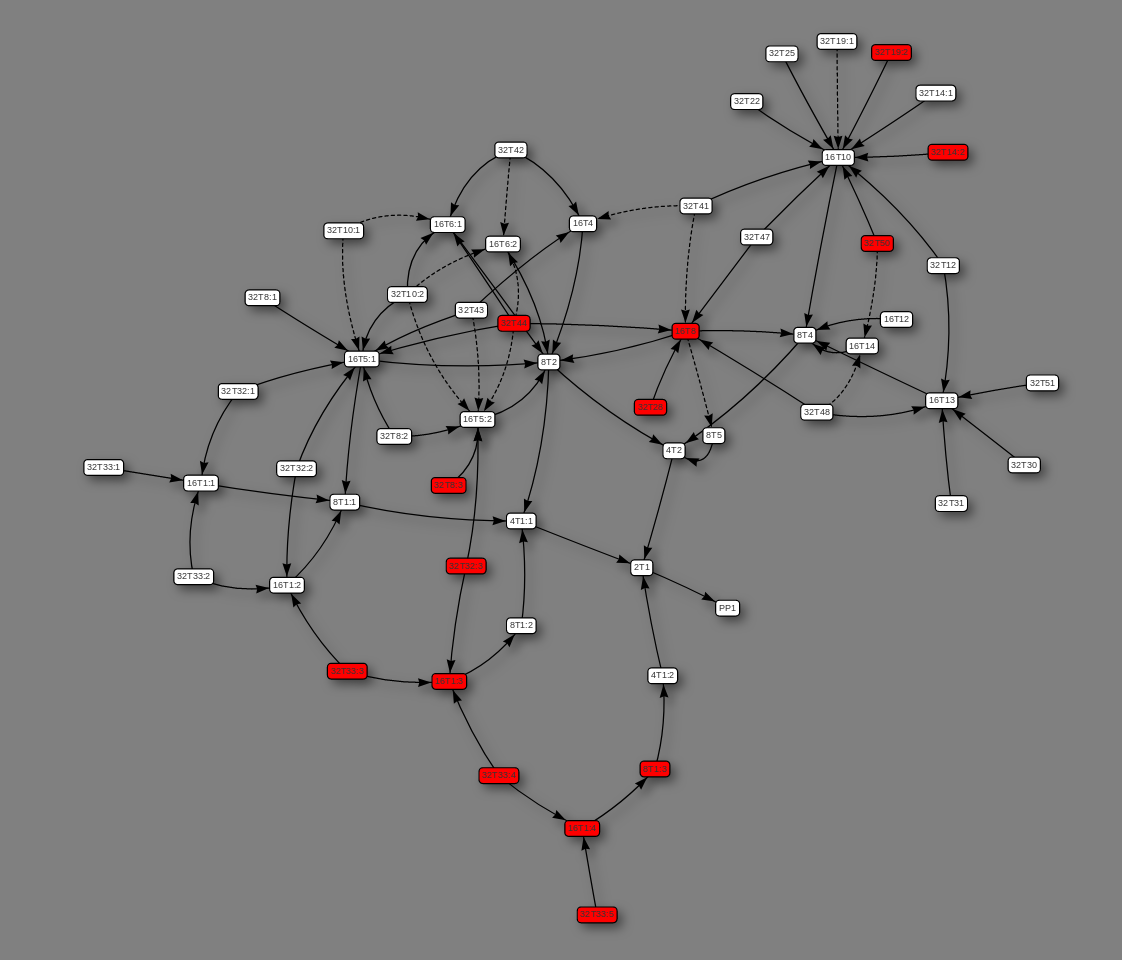
\includegraphics[scale=0.2]{32nh.png}
        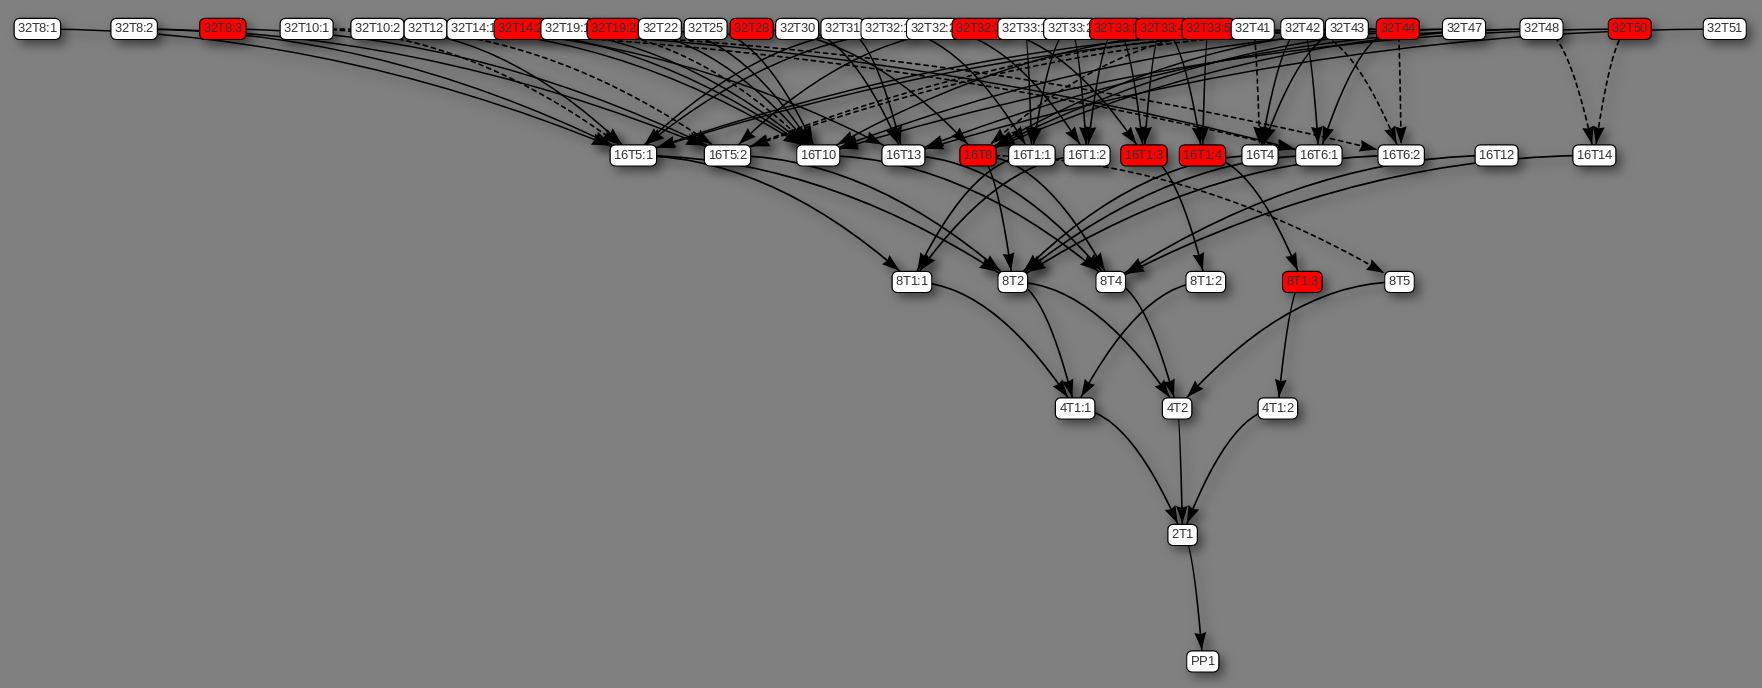
\includegraphics[scale=0.17]{32.png}
      \end{center}
    \end{frame}
  }
  \section{A refined conjecture}{
    \begin{frame}{Passports}
      Recall that a passport $\mathcal{P}$
      consists of the data
      $(g,G,\lambda)$
      where $g\in\ZZ_{\geq 0}$,
      $G$ is a transitive subgroup of $S_d$
      and $\lambda = (\lambda_0,\lambda_1,\lambda_\infty)$
      is a triple of partitions of $d$
      corresponding to conjugacy classes $(C_0,C_1,C_\infty)$
      of $S_d$.
      \pause\par
      The size of
      $\mathcal{P}$ is the cardinality of the
      set
      $\Sigma_\mathcal{P}$
      defined by
      \[
        \Big\{
          (\sigma_0,\sigma_1,\sigma_\infty)\in C_0\times C_1\times C_\infty :
          \sigma_\infty\sigma_1\sigma_0=1
          \text{ and }
          \langle\sigma_0,\sigma_1\rangle=G
        \Big\}/\!\!\sim
      \]
      where $\sim$ denotes simultaneous conjugation in $S_d$.
      \pause\par
      As a result of the action of
      $G_\QQ$ on $\mathcal{P}$,
      the size of $\mathcal{P}$ bounds the degree of the field
      of moduli of any Belyi map with passport
      $\mathcal{P}$.
      \pause\par
      To instead analyze
      $\Gal(\QQal\,|\,\QQab)$
      we \emph{refine} the notion of a passport.
    \end{frame}
    \begin{frame}{Refined passports}
      A \textbf{refined passport} $\mathscr{P}$
      consists of the data
      $(g,G,c)$
      where $g\in\ZZ_{\geq 0}$,
      $G$ is a transitive subgroup of $S_d$
      and $c = (c_0,c_1,c_\infty)$
      is a triple of conjugacy classes
      of $G$.
      \pause\par
      The size of
      $\mathscr{P}$ is the cardinality of the
      set
      $\Sigma_\mathscr{P}$
      defined by
      \[
        \Big\{
          (\sigma_0,\sigma_1,\sigma_\infty)\in c_0\times c_1\times c_\infty :
          \sigma_\infty\sigma_1\sigma_0=1
          \text{ and }
          \langle\sigma_0,\sigma_1\rangle=G
        \Big\}/\!\!\sim
      \]
      where
      $(\sigma_0,\sigma_1,\sigma_\infty)\sim
      (\sigma_0',\sigma_1',\sigma_\infty')$
      if there exists $\alpha\in\Aut(G)$
      with $\alpha(\sigma_s) = \sigma_s'$ for
      every $s\in\{0,1,\infty\}$.
      \pause\par
      As was the case with passport,
      every permutation triple $\sigma$
      determines a refined passport
      $\mathscr{P}(\sigma)$.
    \end{frame}
    \begin{frame}{A refined conjecture}
      \begin{thm}[M.]
        \vspace{1pt}
        The size of $\mathscr{P}(\sigma)$ is
        equal to $1$ for every
        $2$-group permutation triple
        $\sigma$ with degree $\leq 256$.
      \end{thm}
      \pause\par
      \begin{conj}[ARC]
        \vspace{1pt}
        The size of $\mathscr{P}(\sigma)$ is
        equal to $1$ for every
        $2$-group permutation triple.
      \end{conj}
      \pause\par
      \begin{thm}[M.]
        \vspace{1pt}
        ARC is true for $2$-group permutation triples $\sigma$
        with $\langle\sigma\rangle$ dihedral.
      \end{thm}
    \end{frame}
  }
  \section{Computing equations}{
    \begin{frame}[fragile]{$2$-group Belyi maps as iterated quadratic extensions}
      \begin{center}
        \begin{tikzpicture}[scale=1]
          \node at (0,0) (X0) {$X_0 = \PP^1$};
          \node [above left=of X0] (X1) {$X_1$};
          \node [above =of X1] (X2) {$X_2$};
          \node [above =of X2] (dots) {$\vdots$};
          \node [above =of dots] (Xr) {$X_r$};
          %\draw[<->] (X1) to node [above,rotate=-35] {$\sim$} node {} (X0);
          \draw[->] (X1) to node [below] {$2$} node {} (X0);
          \draw[->] (X2) to node [left] {$2$} node {} (X1);
          \draw[->, bend left] (X2) to node [below, left] {} node {} (X0);
          \draw[->] (dots) to node [left] {$2$} node {} (X2);
          \draw[->] (Xr) to node [left] {$2$} node {} (dots);
          \draw[->, bend left] (Xr) to node [below, left] {} node {} (X0);
          \node at (6,0) (KX0) {$K(X_0) = K(\PP^1)$};
          \node [above left=of KX0] (KX1) {$K(X_1)$};
          \node [above =of KX1] (KX2) {$K(X_2)$};
          \node [above =of KX2] (dots) {$\vdots$};
          \node [above =of dots] (KXr) {$K(X_r)$};
          %\draw[<->] (X1) to node [above,rotate=-35] {$\sim$} node {} (X0);
          \draw[-] (KX1) to node [below] {$2$} node {} (KX0);
          \draw[-] (KX2) to node [left] {$2$} node {} (KX1);
          \draw[-, bend left] (KX2) to node [below, left] {} node {} (KX0);
          \draw[-] (dots) to node [left] {$2$} node {} (KX2);
          \draw[-] (KXr) to node [left] {$2$} node {} (dots);
          \draw[-, bend left] (KXr) to node [below, left] {} node {} (KX0);
        \end{tikzpicture}
      \end{center}
    \end{frame}
    \begin{frame}{A motivating example : setup}
      Let $F$ be a number field with
      integers $\ZZ_F$.
      Let $\Pl(F)$ denote the places of $F$
      and $S_\infty$ the archimedean places.
      For $v\in\Pl(F)\setminus S_\infty$ let
      $\mathfrak{p}_v$ denote the prime ideal
      of $\ZZ_F$ corresponding to $v$.
      \pause\par
      Let $S\subset\Pl(F)\setminus S_\infty$ and let
      $\mathfrak{a} \colonequals\prod_{v\in S}\mathfrak{p}_v$.
      \pause\par
      \begin{ques}
        \vspace{1pt}
        How do we construct a quadratic extension of $F$
        with ramification prescribed by $\mathfrak{a}$?
      \end{ques}
      \pause
      First, it is possible that no such extension exists.
      \pause\par
      Second, if $\mathfrak{a}=(d)$ is principal,
      then $F(\sqrt{d})$ is ramified exactly at
      the $\mathfrak{p}_v$, and $d$ is unique up
      to a unit.
      \pause\par
      If $\mathfrak{a}$ is not principal,
      then the question requires more care.
    \end{frame}
    \begin{frame}{A motivating example : class group}
      Let $\Cl_F$ denote the class group of $F$
      and suppose $\mathfrak{a}\mathfrak{b}^2=(d)$.
      \pause\par
      Then
      $[\mathfrak{a}]=[\mathfrak{b}^{-2}]$
      implies $\mathfrak{a}\in\Cl_F^2$.
      \pause\par
      If we let $[\mathfrak{c}]\in\Cl_F[2]$,
      then
      $[\mathfrak{a}\mathfrak{b}^2]
        =[\mathfrak{a}\mathfrak{b}^2][\mathfrak{c}^2]
        =[\mathfrak{a}(\mathfrak{b}\mathfrak{c})^2]$.
      \pause\par
      To summarize,
      in the case where $\mathfrak{a}$ is not principal
      but there exists $\mathfrak{b}$ with
      $\mathfrak{a}\mathfrak{b}^2$ principal
      we have
      $[\mathfrak{a}]\in\Cl_F^2$
      and $[\mathfrak{b}]$ is unique
      up to multiplication by
      $[\mathfrak{c}]\in\Cl_F[2]$.
      \pause\par
      Given $\mathfrak{a}$ encoding ramification data,
      we want to find $\mathfrak{b}^2$ and $d$
      such that $\mathfrak{a}\mathfrak{b}^2=(d)$.
      \pause\par
      The algorithms in this section
      rely on transporting this technique
      to the function field setting.
    \end{frame}
    \begin{frame}{Algorithm in characteristic $p\geq 3$ : setup}
      We want to do computations modulo primes,
      so we need to think about Belyi maps not over
      $\CC$ or $\QQal$, but over finite fields in
      an analogous way.
      \pause\par
      A Belyi map $\phi\colon X\to\PP^1$ over a field of
      characteristic $p$ where $p\nmid\#\Mon(\phi)$
      is called \textbf{tame}.
      The theory of tame Belyi maps is the same as in
      characteristic zero.
      \pause\par
      Let $F$ be a function field with
      field of constants $\FF_q$
      with $q=p^r$ and $p$ an odd prime.
      Let $\FF_q(x)$ denote the rational function field
      in the variable $x$.
      \pause\par
      A \textbf{$2$-group Belyi map modulo $q$}
      is a Galois extension of function fields
      $\FF_q(x)\hookrightarrow F$
      with $[F:\FF_q(x)]$ a power of $2$
      unramified outside $\{0,1,\infty\}$
      with $p\geq 3$.
    \end{frame}
    \begin{frame}{Algorithm in characteristic $p\geq 3$ : outline}
      We now discuss the broad strokes of the algorithm
      before illustrating how it works with an example.
      \pause
      \begin{enumerate}
        \item
          \textbf{Input}:
          $F$ a $2$-group Belyi map modulo $q$ with
          passport $(g,G,(a,b,c))$,
          $G$ explicitly identified with
          $\Gal(F\,|\,\FF_q(x))$,
          and a triple $(r_0,r_1,r_\infty)\in\{0,1\}^3$.
          \pause
        \item
          Compute $R\colonequals r_0R_0+r_1R_1+r_\infty R_\infty$
          encoding ramification.
          \pause
        \item
          Compute $\Pic(F) = T\oplus\ZZ$
          and let $[R]\in\Pic(F)$.
          % denote the
          % image of $R$ in $\Pic(F)$.
          \pause
        \item
          For each $[a]\in\Pic(F)[2]$ compute
          $D_a\in\Div(F)$ corresponding to
          $[a]+[R]/2$.
          \pause
        \item
          Search for functions
          $f_a\in\mathscr{L}(R-2D_a)$.
          \pause
        \item
          Compute quadratic extensions
          $F(\sqrt{f_a})$ and use
          the explicit automorphisms of $F$
          to test if $F(\sqrt{f_a})$ is Galois.
          \pause
        \item
          Lift automorphisms to identify
          the passports of the
          Galois extensions $F(\sqrt{f_a})$.
      \end{enumerate}
    \end{frame}
    \begin{frame}{Notation for examples}
      \begin{equation*}
        \texttt{DNG-a,b,c-gE-H}
      \end{equation*}
      \begin{align*}
        \texttt{D} &:\text{ degree in }
        \{2,4,8,16,32,64,128,256\}\\
        \texttt{N} &:\text{ either \texttt{T}
        or \texttt{S} identifying group
        database}\\
        \texttt{G} &:\text{ a positive integer
        identifying the group}\\
        \texttt{a} &:\text{ ramification index
        of $0$ in }
        \{2,4,8,16,32,64,128,256\}\\
        \texttt{b} &:\text{ ramification index
        of $1$ in }
        \{2,4,8,16,32,64,128,256\}\\
        \texttt{c} &:\text{ ramification index
        of $\infty$ in }
        \{2,4,8,16,32,64,128,256\}\\
        \texttt{g} &:\text{ just the letter 
        \texttt{g}}\\
        \texttt{E} &:\text{ the genus in }
        \ZZ_{\geq 0}\\
        \texttt{H} &:\text{ the hash
        of the $2$-group permutation triple 
        a positive integer}
      \end{align*}
      \pause
      To identify a passport we omit the hash.
    \end{frame}
    \begin{frame}{Algorithm in characteristic $p\geq 3$ : example}
      % before doing an example we introduce some notation
      % hyperelliptic with 2-torsion field computed?
      \texttt{8T2-4,2,4-g1} : \texttt{8T2} $=\ZZ/4\ZZ\times\ZZ/2\ZZ$
      \newline
      \texttt{16T4-4,4,4-g3} : \texttt{16T4} $=\ZZ/4\ZZ\times\ZZ/4\ZZ$
      \pause\par
      $\texttt{8T2-4,2,4-g1} : F = \FF_3[x](\alpha)=\frac{\FF_3(x)[y]}{(y^8 + (x^3 + x^2 + 2x)y^4 + x^6)}$
      \pause\par
      $\Pic(F) = \ZZ/4\ZZ\oplus\ZZ =
      \langle t\rangle\oplus\langle z\rangle$
      \pause\par
      Group theory tells us that we should be able to obtain
      \texttt{16T4-4,4,4-g3} as a quadratic extension
      of $F$.
      \pause\par
      $R = R_1$, $[R] = 4z\in 2\Pic(F)$, $[a]=2t\in\Pic(F)[2]$
      \pause\par
      Computing $\mathscr{L}(R-2D_a)$ where
      $[D_a] = [a]+[R]/2$ we obtain
      \[
        f = \frac{\alpha^6 + 2x\alpha^4 + (2x^3 + 2x)\alpha^2 + (2x^3 + 2x^2)\alpha + x^4 + 2x^3}{x^3(x+1)}
      \]
      \pause
      \texttt{16T4-4,4,4-g3} : $F(\sqrt{f})$
      % y^2 + 2/(x^4 + x^3)*a^6 + 1/(x^3 + x^2)*a^4 + (x^2 + 1)/(x^3 + x^2)*a^2 + 1/x*a + (2*x + 1)/(x + 1)
    \end{frame}
    \begin{frame}{Algorithm in characteristic $p\geq 3$ : example}
      $F(\sqrt{f}) = \FF_3(x)(\alpha)$ where $\alpha$ satisfies
      \begin{align*}
        &y^{16} + (x^7 + 2x^6 + x^5)y^{14} + (x^{16} + 2x^{14} + x^{13} + 2x^{11})y^{12}\\
        &+ (x^{23} + x^{21} + 2x^{20} + 2x^{18} + x^{17} + x^{15})y^{10}\\
        &+ (x^{31} + 2x^{30} + 2x^{29} + 2x^{28} + x^{27} + 2x^{26} + x^{25} + 2x^{24} + x^{23} + x^{20})y^8\\
        &+ (2x^{38} + 2x^{36} + x^{35} + 2x^{29} + 2x^{27} + x^{26})y^6\\
        &+ (x^{48} + 2x^{47} + 2x^{46} + 2x^{44} + 2x^{43} + 2x^{42}\\
        &\;\;\;\;\;\;\;\;\;\;\,+x^{39} + 2x^{38} + 2x^{37} + 2x^{35} + 2x^{34} + 2x^{33})y^4\\
        &+ (x^{54} + x^{52} + x^{51} + x^{50} + x^{49} + x^{47}\\
        &\;\;\;\;\;\;\;\;\;\;\,+ x^{45} + x^{43} + x^{42} + x^{41} + x^{40} + x^{38})y^2\\
        &+ x^{64} + 2x^{62} + x^{61} + 2x^{59} + 2x^{58} + x^{56}\\
        &+ x^{52} + 2x^{50} + 2x^{49} + x^{47} + 2x^{46} + x^{44}
      \end{align*}
    \end{frame}
    \begin{frame}{Algorithm in characteristic $p\geq 3$ : compute entire passport}
      One issue with our technique
      to compute $2$-group Belyi maps
      is that it only guarantees that the
      resulting Belyi map has the desired
      \emph{passport} and does not allow us
      to control which \emph{isomorphism class} we get.
      \pause\par
      To recover from this we use isomorphism testing
      of function fields to determine if we have
      redundant Belyi maps with a given passport.
      \pause\par
      Since we know the sizes of passports from our
      work with permutation triples,
      we know that we have representatives from
      every isomorphism class
      even if we cannot match the Belyi maps
      to their corresponding permutation triples.
    \end{frame}
    \begin{frame}{Implementation in characteristic zero}
      Our inability to compute $\Pic(F)$
      for $F$ over a number field requires
      us to resort to adhoc techniques in this setting.
      \pause\par
      The only difference from the tame case is that
      without $\Pic(F)$, there is no systematic way
      to find the candidate functions to extract
      a square root.
      \pause\par
      However, we do have access to the ramification points
      of the Belyi maps and instead use combinations
      of these points to try to build a candidate function.
      \pause\par
      Although this implementation does not allow us
      to compute all $2$-group Belyi maps for a given
      degree, it does work well in practice.
    \end{frame}
    \begin{frame}{Results}
      % These algorithms are implemented and available at
      % \begin{center}
        \url{https://github.com/michaelmusty/2GroupDessins}
      % \end{center}
      \begin{itemize}
        \item
          \emph{all} $2$-group Belyi maps modulo $3$ up to degree $32$
        \item
          hundreds of $2$-group Belyi maps up to degree $256$
      \end{itemize}
    \end{frame}
  }
  \begin{frame}{Future work}
    \begin{itemize}
      \item
        higher degree over $\FF_3$
      \item
        non-Galois setting
      \item
        an algorithm in characteristic zero
      \item
        prove ARC for other families of $2$-groups
      \item
        $p$-group Belyi maps for $p$ odd
      \item
        compute torsion fields
    \end{itemize}
  \end{frame}
  \begin{frame}{Acknowledgements}
    \begin{itemize}
      \item
        Dave, Tom, Carl, and John
      \item
        Sam, Jeroen, Edgar, Florian, and Richard
      \item
        Mary, Jim, Matt, and Nicole
    \end{itemize}
    \pause
    \begin{center}
      {\Huge Thanks for listening!}
    \end{center}
  \end{frame}
  \appendix
  % BACKUP SLIDES
  \begin{frame}{The graph of $2$-group Belyi maps}
    \url{https://math.dartmouth.edu/~mjmusty/32.html}
    \newline
    \url{https://math.dartmouth.edu/~mjmusty/32nh.html}
    \begin{center}
      % 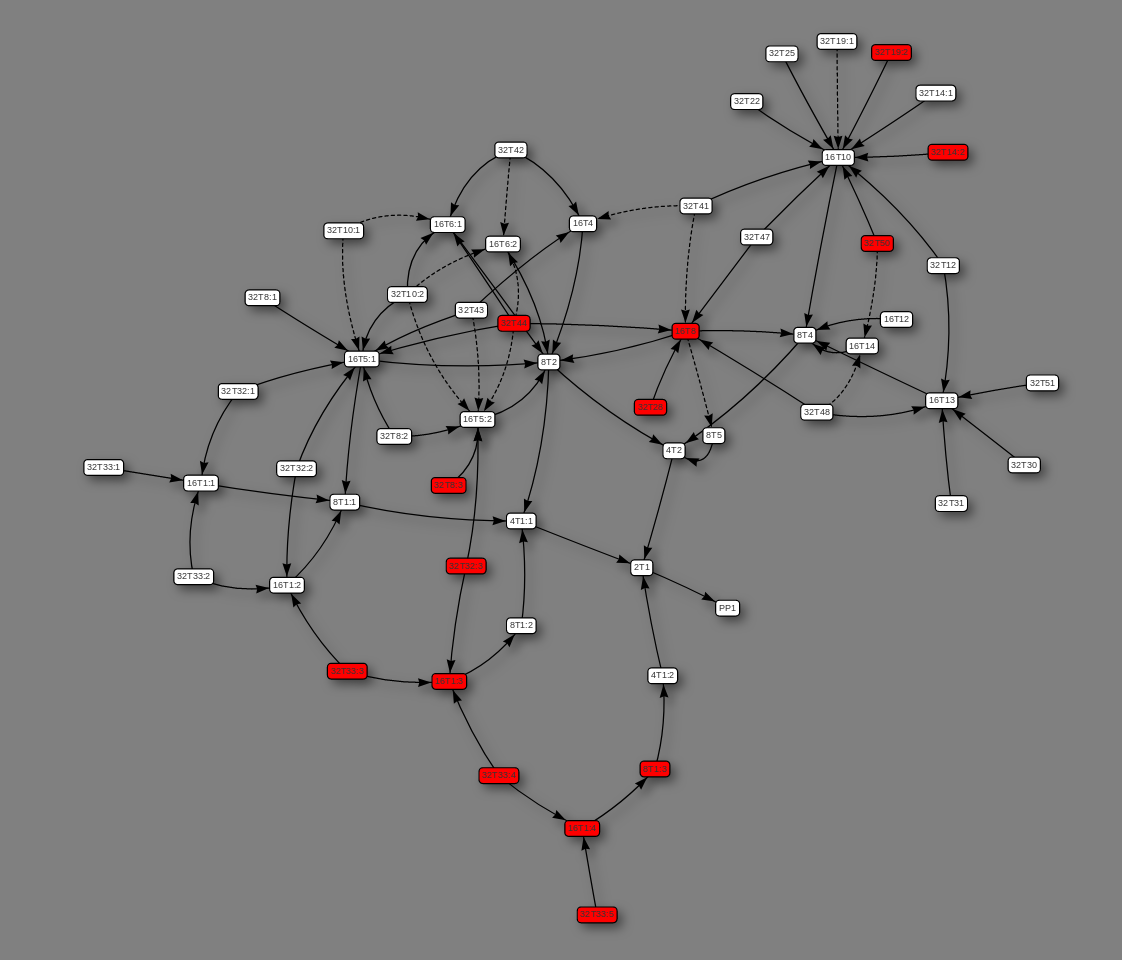
\includegraphics[scale=0.2]{32nh.png}
      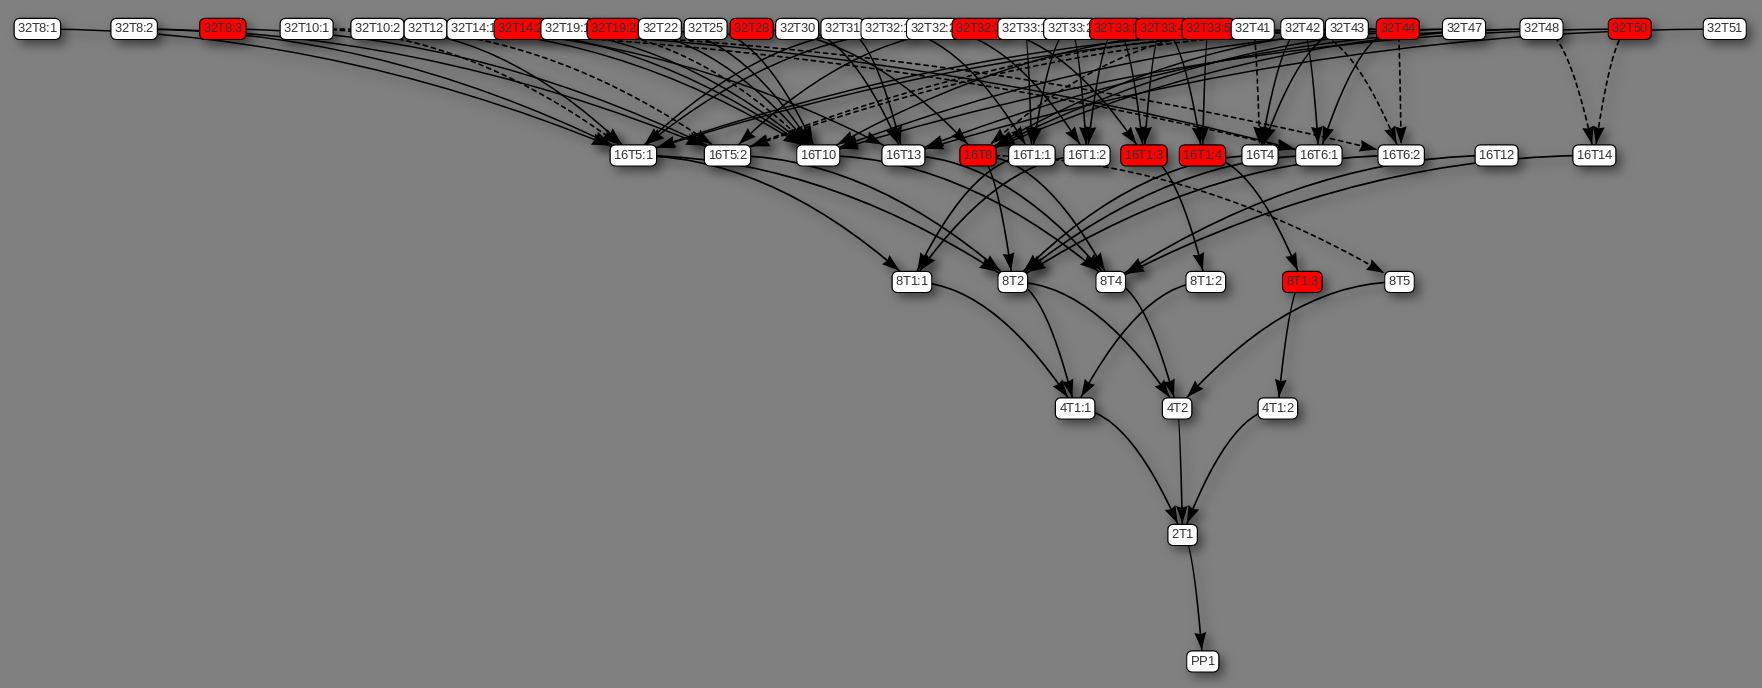
\includegraphics[scale=0.17]{32.png}
    \end{center}
  \end{frame}
  \begin{frame}{Galois representations}
    Let $X$ be an irreducible, smooth
    projective algebraic curve of genus $g\geq 1$
    over a number field $K$.
    Let $G_K\colonequals\Gal(\Kal\,|\,K)$ be
    the absolute Galois group of $K$ and
    let $\ell\in\ZZ$ be prime.
    % \pause\newline
    \newline
    Let $J\colonequals\Jac(X)$ be the
    \textbf{Jacobian variety} of $X$.
    $J$ is an abelian variety of dimension $g$.
    % \pause\newline
    \newline
    $G_K$ acts on the $\ell$-torsion points
    $J[\ell](\Kal)\cong(\ZZ/\ell\ZZ)^{2g}$ of $X$.
    % \pause\newline
    \newline
    This action determines a
    \textbf{mod-$\ell$ Galois representation}
    \[
      \rho\colon G_K\to\Aut(J[\ell])\cong\GL_{2g}(\ZZ/\ell\ZZ).
    \]
    % \pause
    The geometry of $X$ and the arithmetic of
    $\rho$ are inimately related.
    % \pause
    For example,
    if $X$ has good reduction at a prime
    $\mathfrak{p}$ above
    $p\neq\ell$,
    then $\mathfrak{p}$
    will be unramified in the
    \textbf{$\ell$-torsion field}
    $K(J[\ell])$.
  \end{frame}
  \begin{frame}[fragile]{Isomorphism of Belyi maps}
    Let $\phi\colon X\to\PP^1$
    and
    $\phi'\colon X\,'\to\PP^1$
    be Belyi maps of degree $d$.
    % \pause\newline
    \newline
    $\phi$ and $\phi'$ are
    \textbf{isomorphic}
    (respectively \textbf{lax isomorphic})
    if the diagrams
    \[
      \begin{tikzcd}
        X\arrow{rr}{\sim}\arrow{dr}[swap]{\phi}
        &
        &X\,'\arrow{dl}{\phi'}\\
        &\PP^1
      \end{tikzcd},
      \text{ respectively }
      \begin{tikzcd}
        X\arrow{r}{\sim}\arrow{d}[swap]{\phi}&X\,'\arrow{d}{\phi'}\\
        \PP^1\arrow{r}{\sim}[swap]{\beta}&\PP^1
      \end{tikzcd}
    \]
    commute
    where $\beta(\{0,1,\infty\}) = \{0,1,\infty\}$.
  \end{frame}
  \begin{frame}{Algebraic function fields : setup}
    Let $K$ be a perfect field.
    An \textbf{algebraic function field in one variable over $K$}
    is a field extension $F$ over $K$ such that there exists
    $x\in F$ transcendental over $K$ and
    $[F:K(x)]$ is finite.
    % \pause\par
    \par
    $K$ is the \textbf{constant field} of $F$
    and the \textbf{exact constant field} of $F$
    is the algebraic closure of $K$ in $F$.
    % \pause\par
    \par
    As an example,
    let $X$ be an irreducible affine plane curve
    (possibly singular)
    defined by the equation $f(x,y)=0$
    with $f\in K[x,y]$.
    Then the
    \textbf{function field of $X$},
    denoted $K(X)$ is the field of fractions
    of the coordinate ring $K[x,y]/(f(x,y))$
    of $X$.
    % \pause\par
    \par
    A \textbf{place} of $F$ is the maximal ideal
    of some DVR
    $\mathcal{O}_P$ of $F$.
    The valuation on $F$ corresponding to $P$ is
    denoted $\ord_P$.
    % \pause\par
    \par
    The set of places of $F$ is denoted
    $\Pl(F)$ and the \textbf{degree}
    of $P$ is the index
    $[\mathcal{O}_P/P:K]$ of the
    \textbf{residue class field}.
  \end{frame}
  \begin{frame}{Algebraic function fields : Picard group and $\mathscr{L}(D)$}
    The \textbf{divisor class group}
    $\Div(F)$ of $F$ is the free abelian group
    generated by the places of $F$.
    A \textbf{divisor} $D\in\Div(F)$ is represented by
    a sum of places $\sum_{P}a_PP$
    and the \textbf{degree}
    of $D$ is $\sum_{P}a_P\deg(P)$.
    \newline
    The set of \textbf{degree zero divisors} is denoted
    $\Div^0(F)$.
    % \pause\par
    \par
    The image of $\ddiv\colon F^\times\to\Div(F)$ defined by
    % \[
    $
      \ddiv(f) = \sum_{P}\ord_P(f)P
    $
    % \]
    is the subgroup of
    \textbf{principal divisors} of $F$
    denoted $\Princ(F)$.
    % \pause\par
    \par
    The \textbf{Picard group} of $F$ is
    $\Pic(F)\colonequals\Div(F)/\Princ(F)$.
    \newline
    The \textbf{Jacobian} of $F$ is
    $\Pic^0(F)\colonequals\Div^0(F)/\Princ(F)$.
    % \pause\par
    \par
    There is a partial order on $\Div(F)$
    defined by $D_1\geq D_2$ if
    $\ord_P(D_1)\geq\ord_P(D_2)$ for
    every $P\in\Pl(F)$.
    % \pause\par
    \par
    The \textbf{Riemann-Roch space} of a divisor
    $D\in\Div(F)$ is defined by
    $\mathscr{L}(D)\colonequals\{f\in F : \ddiv(f)+D\geq 0\}\cup\{0\}$.
  \end{frame}
  \begin{frame}{Algebraic function fields : quadratic extensions}
    \begin{lem}
      \vspace{1pt}
      Let $aF^{\times 2}$ be a nontrivial coset of
      $F^\times/F^{\times 2}$ and consider the
      extension $L\colonequals F(\sqrt{a})$.
      Then a prime $P$ of $F$ is
      ramified in $L$
      if and only if
      $\ord_P(a)$ is odd.
    \end{lem}
    % \pause
    We now revisit the question of finding a quadratic extension
    of $F(\sqrt{a})$ of $F$ with ramification prescribed
    by $R\in\Div(F)$.
    % \pause\par
    \par
    The simple cases are when no such $a$ exists
    or when $R$ is principal.
    The last case occurs when there exists
    $D$ such that $R-2D=\ddiv(a)$ for some $a\in F$.
    % \pause\par
    \par
    As in the number field setting, this implies
    $R\in 2\Pic(F)$ and $D$ is unique up to
    addition by $T\in\Pic^0(F)[2]$.
  \end{frame}
  \begin{frame}{Algorithm in characteristic $p\geq 3$ : Galois test}
    \textbf{Input}:
    \begin{itemize}
      \item
        $F$ a Galois extension of $\FF_q(x)$
      \item
        $\Gal(F\,|\,\FF_q(x))$ explicitly given as automorphisms of $F$
      \item
        $a\in F$
    \end{itemize}
    \textbf{Output}:
    True if $F(\sqrt{a})$ is Galois over $\FF_q(x)$
    and False otherwise
    % \pause\par
    \par
    \begin{itemize}
      \item
        For each generator $\sigma\in\Gal(F\,|\,\FF_q(x))$
        test if $\sigma(a)/a$ is a square in $F$
      \item
        Return True if $\sigma(a)/a$ is a square in $F$
        for all generators $\sigma$
        and otherwise return False
    \end{itemize}
    % \pause\par
    \par
    Similarly, we can apply the same test after
    extending the constant field from $\FF_q$
    to $\FF_{q^2}$.
  \end{frame}
  \begin{frame}{Algorithm in characteristic $p\geq 3$ : get candidates}
    \textbf{Input}:
    \begin{itemize}
      \item 
        $F$
        a $2$-group Belyi map modulo $q$
        of degree $d=2^m$
        corresponding to a $2$-group
        permutation triple $\sigma$
      \item
        A passport
        $\mathcal{P}=(\wt{G},(a,b,c))$
        with $\wt{G}$ a $2$-group of order
        $2d$ such that there
        exists a
        $2$-group permutation triple
        $\wt{\sigma}$ with passport
        $\mathcal{P}$
        that is a lift of
        $\sigma$
      \item
        $\Gal(F\,|\,\FF_q(x))\cong
        \langle\sigma\rangle$
        explicitly given
        as automorphisms of $F$
    \end{itemize}
    \textbf{Output}:
    A list of candidate functions
    $\{f_i\}$ with each $f_i\in F$
    such that $F(\sqrt{f_i})$ is a
    $2$-group Belyi map modulo $q$
    with passport $\mathcal{P}$.
  \end{frame}
  \begin{frame}{Algorithm in characteristic $p\geq 3$ : get candidates (steps 1-4)}
    \begin{enumerate}
      \item[1.]
        For $s\in\{0,1,\infty\}$
        compute
        \begin{align*}
          r_s\colonequals
          \begin{cases}
            0&
            \text{ if }
            \order(\sigma_s)=
            \order(\wt{\sigma}_s)\\
            1&
            \text{ if }
            \order(\sigma_s)<
            \order(\wt{\sigma}_s)\\
          \end{cases}
        \end{align*}
        % \pause
      \item[2.]
        Compute
        \begin{equation*}
          R\colonequals
          \sum_{s\in\{0,1,\infty\}}r_sR_s
          \in\Div(F)
        \end{equation*}
        where
        $R_0,R_1,R_\infty$
        are defined to be the supports
        of
        % $\ddiv(\phi)$,
        % $\ddiv(\phi-1)$,
        % and $\ddiv(1/\phi)$
        $\ddiv(x)$,
        $\ddiv(x-1)$,
        and $\ddiv(1/x)$
        respectively.
        % \pause
      \item[3.]
        Compute the abelian group
        $\Pic(F)=T\oplus\ZZ$
        (with $T$ a finite abelian group)
        along with a map
        $\psi\colon\Pic(F)\to\Div(F)$.
        % \pause
      \item[4.]
        Compute
        $[R]\colonequals\psi^{-1}(R)$.
    \end{enumerate}
  \end{frame}
  \begin{frame}{Algorithm in characteristic $p\geq 3$ : get candidates (step 5)}
    \begin{enumerate}
      \item[5.]
        For each $a\in\Pic(F)[2]$ compute the
        following:
        % \pause
        \begin{enumerate}
          \item[(a)]
            Let $D_a\colonequals\psi(a+[R]/2)
            \in\Div(F)$.
            % \pause
          \item[(b)]
            Compute $\mathscr{L}(R-2D_a)$.
            % \pause
          \item[(c)]
            If $\mathscr{L}(R-2D_a)$ has dimension
            $1$, then compute
            $f_a\in F$ with $\ddiv(f_a)$
            generating $\mathscr{L}(R-2D_a)$
            and go to Step 5d
            Otherwise go to the next
            $a\in\Pic(F)[2]$.
            % \pause
          \item[(d)]
            Apply Galois test
            to $F$,
            $\Gal(F\,|\,\FF_q(x))$,
            and $f_a$
            from Step 5c
            to see if $F(\sqrt{f_a})$
            generates a Galois extension.
            If $F(\sqrt{f_a})$ is Galois over
            $\FF_q(x)$ then save $f_a$
            and
            go to the next
            $a\in\Pic(F)[2]$.
            If $F(\sqrt{f_a})$ is not Galois
            over $\FF_q(x)$, then go to
            Step 5e.
            % \pause
          \item[(e)]
            Let $F'$ be the function field
            $F$ after extending the field of
            constants $\FF_q$ to $\FF_{q^2}$.
            Apply Galois test
            to $F'$,
            $\Gal(F'\,|\,\FF_{q^2}(x))$,
            and $f_a$
            (viewed as an element of $F'$)
            from Step 5c
            to see if $F'(\sqrt{f_a})$
            generates a Galois extension.
            If $F(\sqrt{f_a})$ is Galois over
            $\FF_{q^2}(x)$ then save $f_a$.
            Go to the next
            $a\in\Pic(F)[2]$.
        \end{enumerate}
    \end{enumerate}
  \end{frame}
  \begin{frame}{Algorithm in characteristic $p\geq 3$ : get candidates (steps 6-8)}
    \begin{enumerate}
      \item[6.]
        Let $S$ be the set of $f_a$
        saved in Step 5d.
        Let $S'$ be the set of $f_a$
        saved in Step 5e.
        % \pause
      \item[7.]
        \begin{itemize}
          \item
            If $S$ is nonempty,
            then
            for each $f_a\in S$
            compute
            $F(\sqrt{f_a})$,
            \[
              G_a\cong\Gal(F(\sqrt{f_a})\,|\,\FF_q(x)),
            \]
            and let
            $S''=
            \{f_a\in S:G_a\cong\wt{G}\}$.
            % \pause
          \item
            If $S$ is empty,
            then
            for each $f_a\in S'$
            compute
            $F'(\sqrt{f_a})$,
            \[
              G_a\cong\Gal(F'(\sqrt{f_a})\,|\,\FF_{q^2}(x)),
            \]
            and let
            $S''=
            \{f_a\in S':G_a\cong\wt{G}\}$.
            % \pause
        \end{itemize}
      \item[8.]
        Return the list $S''$
    \end{enumerate}
  \end{frame}
\end{document}
